\section{Entwurfsmuster}
\begin{frame}{Das Rad muss nicht neu erfunden werden!}
	\begin{itemize}
		\item Manche Probleme tauchen mit schöner Regelmäßigkeit auf
		\item Wichtigste Kategorien:
		\begin{itemize}
			\item Entkoppelung von Komponenten
			\item Strukturierung von Abstraktionsmöglichkeiten
			\item Vereinfachung der Komponentennutzung
		\end{itemize}
	\end{itemize}

	\begin{block}{Notation}
		\begin{center}
			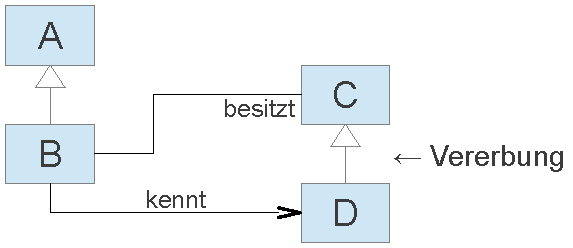
\includegraphics[width=0.7\linewidth]{images/uml-intro.pdf}
		\end{center}
	\end{block}
\end{frame}

\begin{frame}{Wichtige Entwurfsmuster I}
	\begin{block}{Adapter}
		Übersetzt inkompatible Schnittstellen
		\vspace{-0.7em}
		\begin{center}
			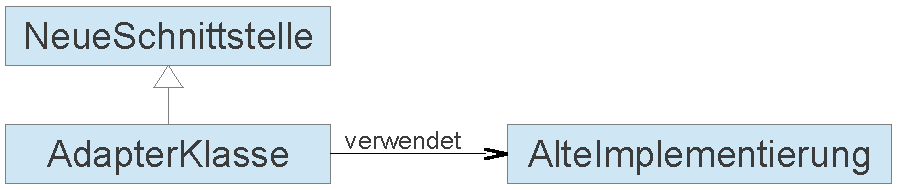
\includegraphics[width=0.85\linewidth]{images/adapter.pdf}
		\end{center}
	\end{block}
	
	\begin{block}{Proxy/Decorator/Wrapper}
		Wird einer anderen Instanz vorgeschaltet und kann diese so kontrollieren oder ihre Funktionalität erweitern		
		\vspace{-0.7em}
		\begin{center}
			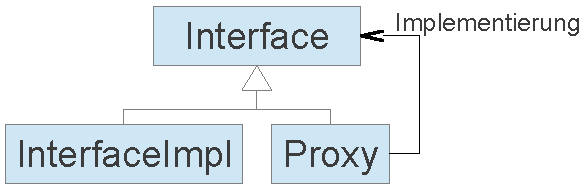
\includegraphics[width=0.6\linewidth]{images/proxy.pdf}
		\end{center}
	\end{block}
\end{frame}
	
\begin{frame}{Wichtige Entwurfsmuster II}
	\begin{block}{Bridge/Pointer to Implementation (Pimpl)}
		Ermöglicht das Entkoppeln von Schnittstelle und Implementierung und erlaubt es, letztere zu verbergen (Information hiding!)
		\vspace{-0.7em}
		\begin{center}
			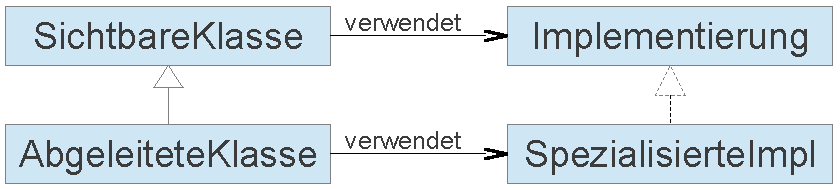
\includegraphics[width=0.85\linewidth]{images/bridge.pdf}
		\end{center}
		\vspace{-1em}
		Implementierungsdetails (\texttt{private}-Bereich!) werden unsichtbar, es bleibt nur ein Zeiger auf eine anonyme Klasse.
		\vspace{-0.5em}		
		\lstinputlisting[basicstyle=\tiny]{cpp-code/pimpl.cpp}
	\end{block}
\end{frame}
	
\begin{frame}{Wichtige Entwurfsmuster III}
	\begin{block}{Observer}
		\begin{itemize}
			\item Benachrichtigung anderer Komponenten über Ereignisse
			\item Die konkreten Implementierungen müssen/sollen sich dabei nicht kennen
		\end{itemize}
		\vspace{-0.7em}
		\begin{center}
			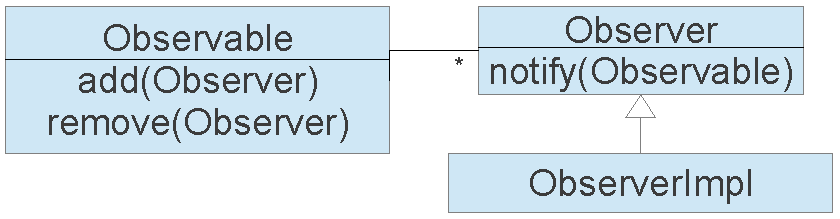
\includegraphics[width=0.85\linewidth]{images/observer.pdf}
		\end{center}
		Sonderfall: Vermittler (Mediator) ähnelt dem Observer
	\end{block}
\end{frame}
	
\begin{frame}{Wichtige Entwurfsmuster IV}
	\begin{block}{Template (Schablonenmethode) und Strategie}
		\begin{itemize}
			\item Schablonenmethoden delegieren die Implementierung einzelner Aspekte an Kindklassen
			\item Das Strategie-Pattern macht komplette Klassen als Gegenstand einer Implementierung austauschbar
		\end{itemize}
		\vspace{-1em}
		\begin{center}
			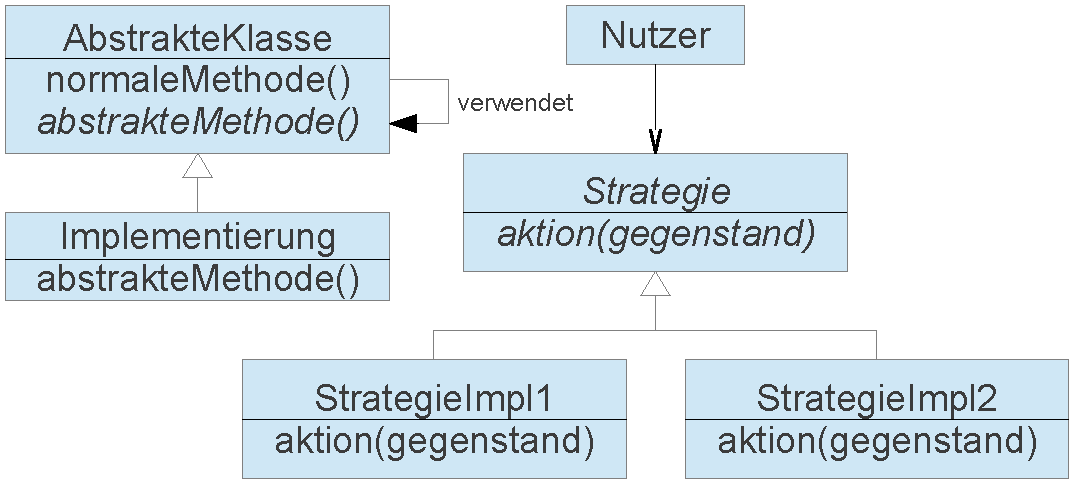
\includegraphics[width=0.85\linewidth]{images/strategy.pdf}
		\end{center}
	\end{block}
\end{frame}

\begin{frame}{Wichtige Entwurfsmuster V}	
	\begin{block}{Factory}
		\begin{itemize}
			\item Klassen oder Methoden, die neue Objekte erzeugen
			\item Interpretierbar als Sonderfall von Template und Strategie
		\end{itemize}		
		\vspace{-1em}
		\begin{center}
			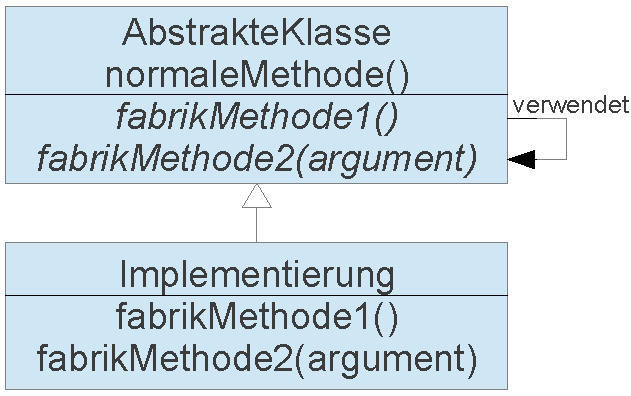
\includegraphics[width=0.6\linewidth]{images/factorymethod.pdf}
		\end{center}		
	\end{block}
\end{frame}

\begin{frame}{Wichtige Entwurfsmuster V}	
	\begin{block}{Abstrakte Factory}
		\begin{center}
			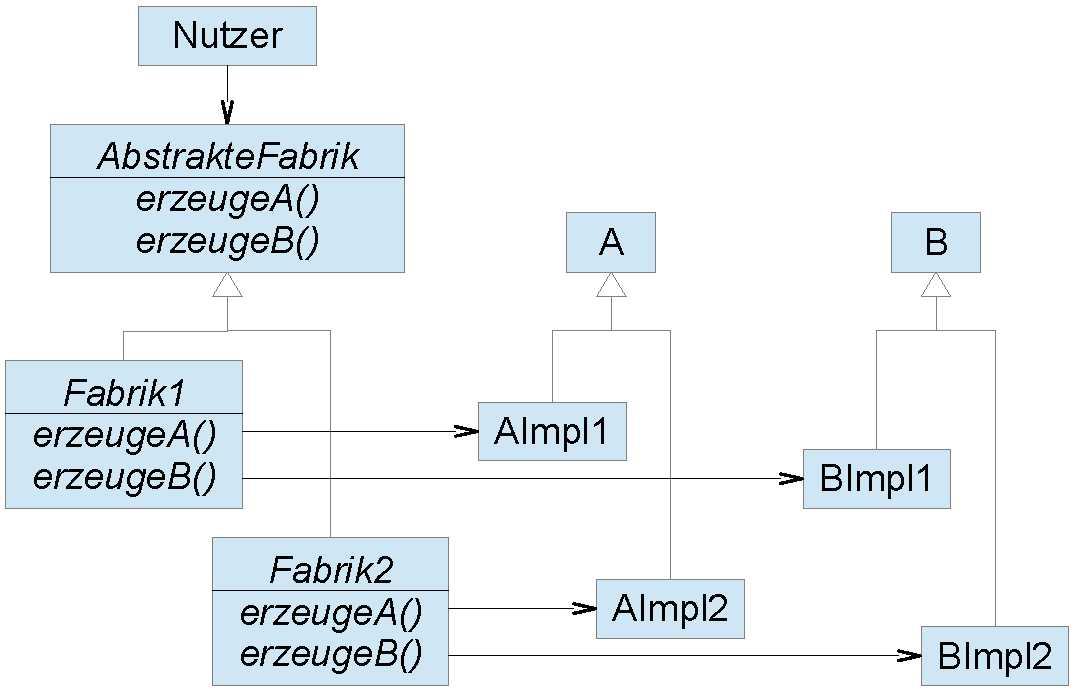
\includegraphics[width=0.85\linewidth]{images/factory.pdf}
		\end{center}		
	\end{block}
\end{frame}

\begin{frame}{Wichtige Entwurfsmuster VI}
	\begin{block}{Fassade}
		Eine Klasse die das (komplizierte) Zusammenspiel innerhalb eines ganzen Subsystems hinter einer einfachen, einheitlichen Schnittstelle verbirgt.
	\end{block}
	
	\begin{block}{Dummy/Null-Objekt}
		Eine Klasse die einfach \enquote{nichts} tut. Solche Objekte können aufwändige Sonderfälle ersetzen.
	\end{block}
\end{frame}

